\documentclass[1p]{elsarticle_modified}
%\bibliographystyle{elsarticle-num}

%\usepackage[colorlinks]{hyperref}
%\usepackage{abbrmath_seonhwa} %\Abb, \Ascr, \Acal ,\Abf, \Afrak
\usepackage{amsfonts}
\usepackage{amssymb}
\usepackage{amsmath}
\usepackage{amsthm}
\usepackage{scalefnt}
\usepackage{amsbsy}
\usepackage{kotex}
\usepackage{caption}
\usepackage{subfig}
\usepackage{color}
\usepackage{graphicx}
\usepackage{xcolor} %% white, black, red, green, blue, cyan, magenta, yellow
\usepackage{float}
\usepackage{setspace}
\usepackage{hyperref}

\usepackage{tikz}
\usetikzlibrary{arrows}

\usepackage{multirow}
\usepackage{array} % fixed length table
\usepackage{hhline}

%%%%%%%%%%%%%%%%%%%%%
\makeatletter
\renewcommand*\env@matrix[1][\arraystretch]{%
	\edef\arraystretch{#1}%
	\hskip -\arraycolsep
	\let\@ifnextchar\new@ifnextchar
	\array{*\c@MaxMatrixCols c}}
\makeatother %https://tex.stackexchange.com/questions/14071/how-can-i-increase-the-line-spacing-in-a-matrix
%%%%%%%%%%%%%%%

\usepackage[normalem]{ulem}

\newcommand{\msout}[1]{\ifmmode\text{\sout{\ensuremath{#1}}}\else\sout{#1}\fi}
%SOURCE: \msout is \stkout macro in https://tex.stackexchange.com/questions/20609/strikeout-in-math-mode

\newcommand{\cancel}[1]{
	\ifmmode
	{\color{red}\msout{#1}}
	\else
	{\color{red}\sout{#1}}
	\fi
}

\newcommand{\add}[1]{
	{\color{blue}\uwave{#1}}
}

\newcommand{\replace}[2]{
	\ifmmode
	{\color{red}\msout{#1}}{\color{blue}\uwave{#2}}
	\else
	{\color{red}\sout{#1}}{\color{blue}\uwave{#2}}
	\fi
}

\newcommand{\Sol}{\mathcal{S}} %segment
\newcommand{\D}{D} %diagram
\newcommand{\A}{\mathcal{A}} %arc


%%%%%%%%%%%%%%%%%%%%%%%%%%%%%5 test

\def\sl{\operatorname{\textup{SL}}(2,\Cbb)}
\def\psl{\operatorname{\textup{PSL}}(2,\Cbb)}
\def\quan{\mkern 1mu \triangleright \mkern 1mu}

\theoremstyle{definition}
\newtheorem{thm}{Theorem}[section]
\newtheorem{prop}[thm]{Proposition}
\newtheorem{lem}[thm]{Lemma}
\newtheorem{ques}[thm]{Question}
\newtheorem{cor}[thm]{Corollary}
\newtheorem{defn}[thm]{Definition}
\newtheorem{exam}[thm]{Example}
\newtheorem{rmk}[thm]{Remark}
\newtheorem{alg}[thm]{Algorithm}

\newcommand{\I}{\sqrt{-1}}
\begin{document}

%\begin{frontmatter}
%
%\title{Boundary parabolic representations of knots up to 8 crossings}
%
%%% Group authors per affiliation:
%\author{Yunhi Cho} 
%\address{Department of Mathematics, University of Seoul, Seoul, Korea}
%\ead{yhcho@uos.ac.kr}
%
%
%\author{Seonhwa Kim} %\fnref{s_kim}}
%\address{Center for Geometry and Physics, Institute for Basic Science, Pohang, 37673, Korea}
%\ead{ryeona17@ibs.re.kr}
%
%\author{Hyuk Kim}
%\address{Department of Mathematical Sciences, Seoul National University, Seoul 08826, Korea}
%\ead{hyukkim@snu.ac.kr}
%
%\author{Seokbeom Yoon}
%\address{Department of Mathematical Sciences, Seoul National University, Seoul, 08826,  Korea}
%\ead{sbyoon15@snu.ac.kr}
%
%\begin{abstract}
%We find all boundary parabolic representation of knots up to 8 crossings.
%
%\end{abstract}
%\begin{keyword}
%    \MSC[2010] 57M25 
%\end{keyword}
%
%\end{frontmatter}

%\linenumbers
%\tableofcontents
%
\newcommand\colored[1]{\textcolor{white}{\rule[-0.35ex]{0.8em}{1.4ex}}\kern-0.8em\color{red} #1}%
%\newcommand\colored[1]{\textcolor{white}{ #1}\kern-2.17ex	\textcolor{white}{ #1}\kern-1.81ex	\textcolor{white}{ #1}\kern-2.15ex\color{red}#1	}

{\Large $\underline{12n_{0851}~(K12n_{0851})}$}

\setlength{\tabcolsep}{10pt}
\renewcommand{\arraystretch}{1.6}
\vspace{1cm}\begin{tabular}{m{100pt}>{\centering\arraybackslash}m{274pt}}
\multirow{5}{120pt}{
	\centering
	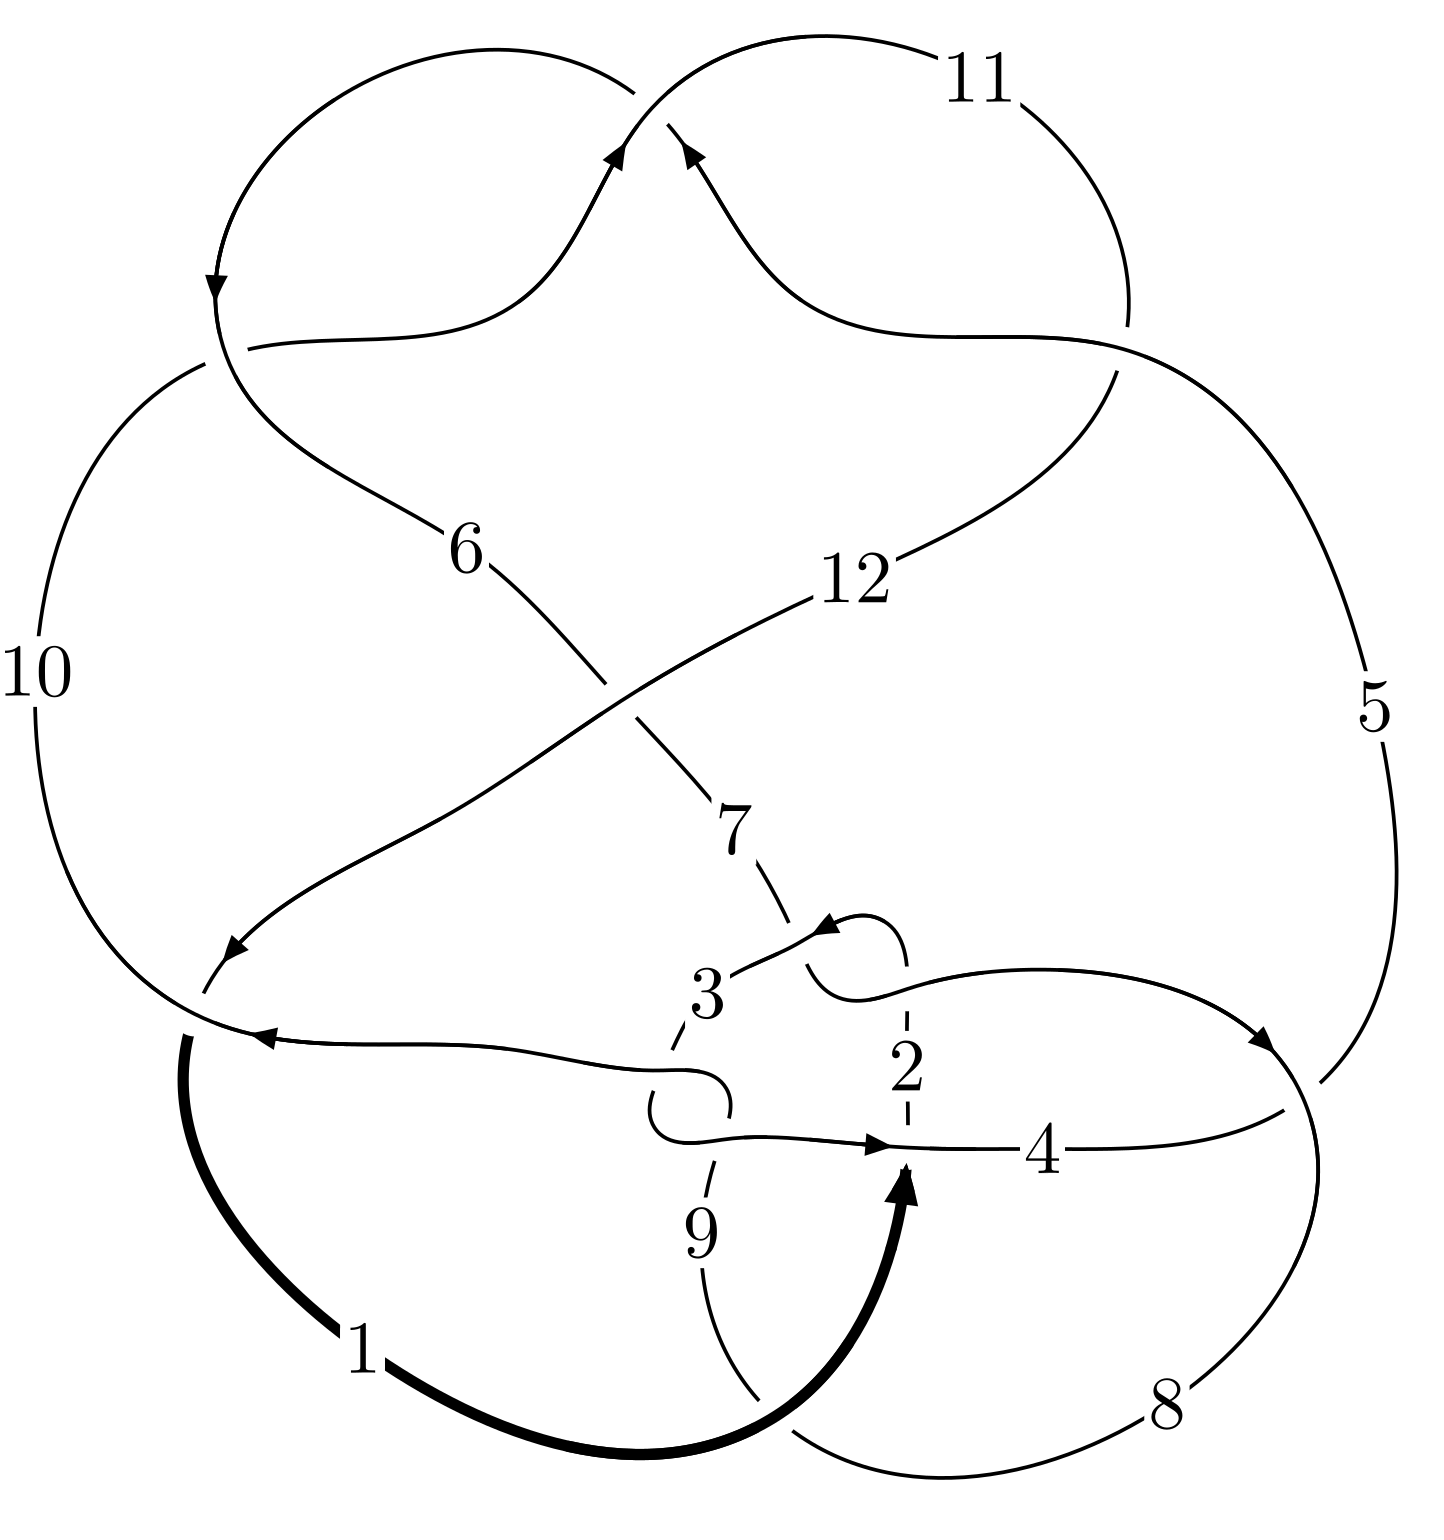
\includegraphics[width=112pt]{../../../GIT/diagram.site/Diagrams/png/2940_12n_0851.png}\\
\ \ \ A knot diagram\footnotemark}&
\allowdisplaybreaks
\textbf{Linearized knot diagam} \\
\cline{2-2}
 &
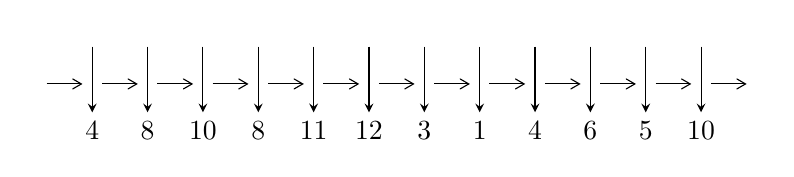
\begin{tikzpicture}[x=20pt, y=17pt]
	% nodes
	\node (C0) at (0, 0) {};
	\node (C1) at (1, 0) {};
	\node (C1U) at (1, +1) {};
	\node (C1D) at (1, -1) {4};

	\node (C2) at (2, 0) {};
	\node (C2U) at (2, +1) {};
	\node (C2D) at (2, -1) {8};

	\node (C3) at (3, 0) {};
	\node (C3U) at (3, +1) {};
	\node (C3D) at (3, -1) {10};

	\node (C4) at (4, 0) {};
	\node (C4U) at (4, +1) {};
	\node (C4D) at (4, -1) {8};

	\node (C5) at (5, 0) {};
	\node (C5U) at (5, +1) {};
	\node (C5D) at (5, -1) {11};

	\node (C6) at (6, 0) {};
	\node (C6U) at (6, +1) {};
	\node (C6D) at (6, -1) {12};

	\node (C7) at (7, 0) {};
	\node (C7U) at (7, +1) {};
	\node (C7D) at (7, -1) {3};

	\node (C8) at (8, 0) {};
	\node (C8U) at (8, +1) {};
	\node (C8D) at (8, -1) {1};

	\node (C9) at (9, 0) {};
	\node (C9U) at (9, +1) {};
	\node (C9D) at (9, -1) {4};

	\node (C10) at (10, 0) {};
	\node (C10U) at (10, +1) {};
	\node (C10D) at (10, -1) {6};

	\node (C11) at (11, 0) {};
	\node (C11U) at (11, +1) {};
	\node (C11D) at (11, -1) {5};

	\node (C12) at (12, 0) {};
	\node (C12U) at (12, +1) {};
	\node (C12D) at (12, -1) {10};
	\node (C13) at (13, 0) {};

	% arrows
	\draw[->,>={angle 60}]
	(C0) edge (C1) (C1) edge (C2) (C2) edge (C3) (C3) edge (C4) (C4) edge (C5) (C5) edge (C6) (C6) edge (C7) (C7) edge (C8) (C8) edge (C9) (C9) edge (C10) (C10) edge (C11) (C11) edge (C12) (C12) edge (C13) ;	\draw[->,>=stealth]
	(C1U) edge (C1D) (C2U) edge (C2D) (C3U) edge (C3D) (C4U) edge (C4D) (C5U) edge (C5D) (C6U) edge (C6D) (C7U) edge (C7D) (C8U) edge (C8D) (C9U) edge (C9D) (C10U) edge (C10D) (C11U) edge (C11D) (C12U) edge (C12D) ;
	\end{tikzpicture} \\
\hhline{~~} \\& 
\textbf{Solving Sequence} \\ \cline{2-2} 
 &
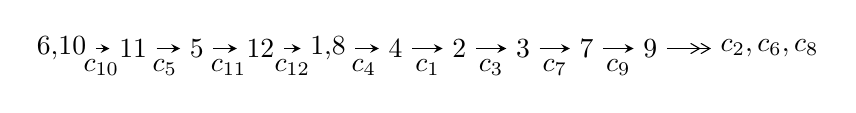
\begin{tikzpicture}[x=23pt, y=7pt]
	% node
	\node (A0) at (-1/8, 0) {6,10};
	\node (A1) at (1, 0) {11};
	\node (A2) at (2, 0) {5};
	\node (A3) at (3, 0) {12};
	\node (A4) at (65/16, 0) {1,8};
	\node (A5) at (41/8, 0) {4};
	\node (A6) at (49/8, 0) {2};
	\node (A7) at (57/8, 0) {3};
	\node (A8) at (65/8, 0) {7};
	\node (A9) at (73/8, 0) {9};
	\node (C1) at (1/2, -1) {$c_{10}$};
	\node (C2) at (3/2, -1) {$c_{5}$};
	\node (C3) at (5/2, -1) {$c_{11}$};
	\node (C4) at (7/2, -1) {$c_{12}$};
	\node (C5) at (37/8, -1) {$c_{4}$};
	\node (C6) at (45/8, -1) {$c_{1}$};
	\node (C7) at (53/8, -1) {$c_{3}$};
	\node (C8) at (61/8, -1) {$c_{7}$};
	\node (C9) at (69/8, -1) {$c_{9}$};
	\node (A10) at (11, 0) {$c_{2},c_{6},c_{8}$};

	% edge
	\draw[->,>=stealth]	
	(A0) edge (A1) (A1) edge (A2) (A2) edge (A3) (A3) edge (A4) (A4) edge (A5) (A5) edge (A6) (A6) edge (A7) (A7) edge (A8) (A8) edge (A9) ;
	\draw[->>,>={angle 60}]	
	(A9) edge (A10);
\end{tikzpicture} \\ 

\end{tabular} \\

\footnotetext{
The image of knot diagram is generated by the software ``\textbf{Draw programme}" developed by Andrew Bartholomew(\url{http://www.layer8.co.uk/maths/draw/index.htm\#Running-draw}), where we modified some parts for our purpose(\url{https://github.com/CATsTAILs/LinksPainter}).
}\phantom \\ \newline 
\centering \textbf{Ideals for irreducible components\footnotemark of $X_{\text{par}}$} 
 
\begin{align*}
I^u_{1}&=\langle 
u^{13}-4 u^{12}+14 u^{11}-32 u^{10}+61 u^9-92 u^8+114 u^7-113 u^6+90 u^5-49 u^4+18 u^3+2 u^2+2 b-5 u,\\
\phantom{I^u_{1}}&\phantom{= \langle  }- u^{13}+5 u^{12}+\cdots+2 a-5,\;u^{14}-6 u^{13}+\cdots+10 u-4\rangle \\
I^u_{2}&=\langle 
u^{11}+5 u^9+9 u^7+5 u^5+u^4-2 u^3+2 u^2+b-2 u,\\
\phantom{I^u_{2}}&\phantom{= \langle  }- u^{11}+u^{10}-5 u^9+5 u^8-9 u^7+9 u^6-5 u^5+4 u^4+3 u^3-4 u^2+a+4 u-2,\\
\phantom{I^u_{2}}&\phantom{= \langle  }u^{12}+6 u^{10}+13 u^8+10 u^6+u^5-2 u^4+3 u^3-4 u^2+2 u+1\rangle \\
\\
\end{align*}
\raggedright * 2 irreducible components of $\dim_{\mathbb{C}}=0$, with total 26 representations.\\
\footnotetext{All coefficients of polynomials are rational numbers. But the coefficients are sometimes approximated in decimal forms when there is not enough margin.}
\newpage
\renewcommand{\arraystretch}{1}
\centering \section*{I. $I^u_{1}= \langle u^{13}-4 u^{12}+\cdots+2 b-5 u,\;- u^{13}+5 u^{12}+\cdots+2 a-5,\;u^{14}-6 u^{13}+\cdots+10 u-4 \rangle$}
\flushleft \textbf{(i) Arc colorings}\\
\begin{tabular}{m{7pt} m{180pt} m{7pt} m{180pt} }
\flushright $a_{6}=$&$\begin{pmatrix}0\\u\end{pmatrix}$ \\
\flushright $a_{10}=$&$\begin{pmatrix}1\\0\end{pmatrix}$ \\
\flushright $a_{11}=$&$\begin{pmatrix}1\\u^2\end{pmatrix}$ \\
\flushright $a_{5}=$&$\begin{pmatrix}u\\u^3+u\end{pmatrix}$ \\
\flushright $a_{12}=$&$\begin{pmatrix}u^2+1\\u^4+2 u^2\end{pmatrix}$ \\
\flushright $a_{1}=$&$\begin{pmatrix}- u^4- u^2+1\\u^4+2 u^2\end{pmatrix}$ \\
\flushright $a_{8}=$&$\begin{pmatrix}\frac{1}{2} u^{13}-\frac{5}{2} u^{12}+\cdots-\frac{7}{2} u+\frac{5}{2}\\-\frac{1}{2} u^{13}+2 u^{12}+\cdots- u^2+\frac{5}{2} u\end{pmatrix}$ \\
\flushright $a_{4}=$&$\begin{pmatrix}\frac{1}{4} u^{13}- u^{12}+\cdots+\frac{3}{4} u-1\\\frac{1}{2} u^{13}-3 u^{12}+\cdots-\frac{9}{2} u+3\end{pmatrix}$ \\
\flushright $a_{2}=$&$\begin{pmatrix}- u^{13}+\frac{11}{2} u^{12}+\cdots+6 u-\frac{5}{2}\\-\frac{1}{2} u^{13}+3 u^{12}+\cdots+\frac{11}{2} u-4\end{pmatrix}$ \\
\flushright $a_{3}=$&$\begin{pmatrix}\frac{3}{4} u^{13}-4 u^{12}+\cdots-\frac{15}{4} u+2\\\frac{1}{2} u^{13}-3 u^{12}+\cdots-\frac{9}{2} u+3\end{pmatrix}$ \\
\flushright $a_{7}=$&$\begin{pmatrix}- u^5-2 u^3- u\\- u^7-3 u^5-2 u^3+u\end{pmatrix}$ \\
\flushright $a_{9}=$&$\begin{pmatrix}- u^{13}+\frac{9}{2} u^{12}+\cdots+4 u-\frac{3}{2}\\\frac{1}{2} u^{13}-2 u^{12}+\cdots+u^2-\frac{3}{2} u\end{pmatrix}$\\&\end{tabular}
\flushleft \textbf{(ii) Obstruction class $= -1$}\\~\\
\flushleft \textbf{(iii) Cusp Shapes $= - u^{13}+6 u^{12}-24 u^{11}+68 u^{10}-151 u^9+270 u^8-394 u^7+469 u^6-448 u^5+327 u^4-164 u^3+34 u^2+24 u-26$}\\~\\
\newpage\renewcommand{\arraystretch}{1}
\flushleft \textbf{(iv) u-Polynomials at the component}\newline \\
\begin{tabular}{m{50pt}|m{274pt}}
Crossings & \hspace{64pt}u-Polynomials at each crossing \\
\hline $$\begin{aligned}c_{1}\end{aligned}$$&$\begin{aligned}
&u^{14}-5 u^{13}+\cdots-2 u+1
\end{aligned}$\\
\hline $$\begin{aligned}c_{2},c_{3},c_{7}\\c_{9}\end{aligned}$$&$\begin{aligned}
&u^{14}- u^{13}+\cdots-2 u-1
\end{aligned}$\\
\hline $$\begin{aligned}c_{4},c_{8}\end{aligned}$$&$\begin{aligned}
&u^{14}+2 u^{13}+\cdots-3 u-1
\end{aligned}$\\
\hline $$\begin{aligned}c_{5},c_{10},c_{11}\end{aligned}$$&$\begin{aligned}
&u^{14}-6 u^{13}+\cdots+10 u-4
\end{aligned}$\\
\hline $$\begin{aligned}c_{6}\end{aligned}$$&$\begin{aligned}
&u^{14}+6 u^{13}+\cdots-462 u-180
\end{aligned}$\\
\hline $$\begin{aligned}c_{12}\end{aligned}$$&$\begin{aligned}
&u^{14}-4 u^{13}+\cdots+1960 u+1216
\end{aligned}$\\
\hline
\end{tabular}\\~\\
\newpage\renewcommand{\arraystretch}{1}
\flushleft \textbf{(v) Riley Polynomials at the component}\newline \\
\begin{tabular}{m{50pt}|m{274pt}}
Crossings & \hspace{64pt}Riley Polynomials at each crossing \\
\hline $$\begin{aligned}c_{1}\end{aligned}$$&$\begin{aligned}
&y^{14}-29 y^{13}+\cdots-38 y+1
\end{aligned}$\\
\hline $$\begin{aligned}c_{2},c_{3},c_{7}\\c_{9}\end{aligned}$$&$\begin{aligned}
&y^{14}+39 y^{13}+\cdots+14 y+1
\end{aligned}$\\
\hline $$\begin{aligned}c_{4},c_{8}\end{aligned}$$&$\begin{aligned}
&y^{14}+30 y^{13}+\cdots-33 y+1
\end{aligned}$\\
\hline $$\begin{aligned}c_{5},c_{10},c_{11}\end{aligned}$$&$\begin{aligned}
&y^{14}+12 y^{13}+\cdots-156 y+16
\end{aligned}$\\
\hline $$\begin{aligned}c_{6}\end{aligned}$$&$\begin{aligned}
&y^{14}-4 y^{13}+\cdots-178524 y+32400
\end{aligned}$\\
\hline $$\begin{aligned}c_{12}\end{aligned}$$&$\begin{aligned}
&y^{14}+76 y^{13}+\cdots-36622528 y+1478656
\end{aligned}$\\
\hline
\end{tabular}\\~\\
\newpage\flushleft \textbf{(vi) Complex Volumes and Cusp Shapes}
$$\begin{array}{c|c|c}  
\text{Solutions to }I^u_{1}& \I (\text{vol} + \sqrt{-1}CS) & \text{Cusp shape}\\
 \hline 
\begin{aligned}
u &= \phantom{-}0.858928\phantom{ +0.000000I} \\
a &= -0.109294\phantom{ +0.000000I} \\
b &= -0.665442\phantom{ +0.000000I}\end{aligned}
 & -6.60134\phantom{ +0.000000I} & -10.5000\phantom{ +0.000000I} \\ \hline\begin{aligned}
u &= -0.057867 + 1.252230 I \\
a &= \phantom{-}0.540753 - 0.387507 I \\
b &= -0.147291 + 0.486948 I\end{aligned}
 & \phantom{-}3.16264 + 1.26178 I & -8.12371 - 5.07005 I \\ \hline\begin{aligned}
u &= -0.057867 - 1.252230 I \\
a &= \phantom{-}0.540753 + 0.387507 I \\
b &= -0.147291 - 0.486948 I\end{aligned}
 & \phantom{-}3.16264 - 1.26178 I & -8.12371 + 5.07005 I \\ \hline\begin{aligned}
u &= \phantom{-}0.606137 + 0.416811 I \\
a &= -0.101897 - 1.053150 I \\
b &= \phantom{-}1.314670 - 0.337317 I\end{aligned}
 & \phantom{-}2.36646 - 1.94252 I & -10.80294 + 5.02822 I \\ \hline\begin{aligned}
u &= \phantom{-}0.606137 - 0.416811 I \\
a &= -0.101897 + 1.053150 I \\
b &= \phantom{-}1.314670 + 0.337317 I\end{aligned}
 & \phantom{-}2.36646 + 1.94252 I & -10.80294 - 5.02822 I \\ \hline\begin{aligned}
u &= \phantom{-}1.116120 + 0.614225 I \\
a &= \phantom{-}0.611664 + 0.699390 I \\
b &= -1.89280 + 0.05423 I\end{aligned}
 & \phantom{-}14.8430 - 3.5814 I & -10.19251 + 1.82347 I \\ \hline\begin{aligned}
u &= \phantom{-}1.116120 - 0.614225 I \\
a &= \phantom{-}0.611664 - 0.699390 I \\
b &= -1.89280 - 0.05423 I\end{aligned}
 & \phantom{-}14.8430 + 3.5814 I & -10.19251 - 1.82347 I \\ \hline\begin{aligned}
u &= \phantom{-}0.396990 + 1.275890 I \\
a &= \phantom{-}0.477782 + 0.520657 I \\
b &= -0.666680 - 0.056910 I\end{aligned}
 & -2.63737 - 4.50416 I & -7.28522 + 5.75195 I \\ \hline\begin{aligned}
u &= \phantom{-}0.396990 - 1.275890 I \\
a &= \phantom{-}0.477782 - 0.520657 I \\
b &= -0.666680 + 0.056910 I\end{aligned}
 & -2.63737 + 4.50416 I & -7.28522 - 5.75195 I \\ \hline\begin{aligned}
u &= \phantom{-}0.22659 + 1.45890 I \\
a &= -2.00625 - 0.57060 I \\
b &= \phantom{-}1.74247 - 0.66474 I\end{aligned}
 & \phantom{-}8.40238 - 5.00923 I & -8.98141 + 6.39703 I\\
 \hline 
 \end{array}$$\newpage$$\begin{array}{c|c|c}  
\text{Solutions to }I^u_{1}& \I (\text{vol} + \sqrt{-1}CS) & \text{Cusp shape}\\
 \hline 
\begin{aligned}
u &= \phantom{-}0.22659 - 1.45890 I \\
a &= -2.00625 + 0.57060 I \\
b &= \phantom{-}1.74247 + 0.66474 I\end{aligned}
 & \phantom{-}8.40238 + 5.00923 I & -8.98141 - 6.39703 I \\ \hline\begin{aligned}
u &= \phantom{-}0.43989 + 1.60061 I \\
a &= \phantom{-}1.72225 + 0.99994 I \\
b &= -1.94337 + 0.15344 I\end{aligned}
 & -17.6523 - 9.3227 I & -8.42289 + 3.11986 I \\ \hline\begin{aligned}
u &= \phantom{-}0.43989 - 1.60061 I \\
a &= \phantom{-}1.72225 - 0.99994 I \\
b &= -1.94337 - 0.15344 I\end{aligned}
 & -17.6523 + 9.3227 I & -8.42289 - 3.11986 I \\ \hline\begin{aligned}
u &= -0.314654\phantom{ +0.000000I} \\
a &= \phantom{-}0.620672\phantom{ +0.000000I} \\
b &= -0.148554\phantom{ +0.000000I}\end{aligned}
 & -0.498688\phantom{ +0.000000I} & -19.8820\phantom{ +0.000000I}\\
 \hline 
 \end{array}$$\newpage\newpage\renewcommand{\arraystretch}{1}
\centering \section*{II. $I^u_{2}= \langle u^{11}+5 u^9+\cdots+b-2 u,\;- u^{11}+u^{10}+\cdots+a-2,\;u^{12}+6 u^{10}+\cdots+2 u+1 \rangle$}
\flushleft \textbf{(i) Arc colorings}\\
\begin{tabular}{m{7pt} m{180pt} m{7pt} m{180pt} }
\flushright $a_{6}=$&$\begin{pmatrix}0\\u\end{pmatrix}$ \\
\flushright $a_{10}=$&$\begin{pmatrix}1\\0\end{pmatrix}$ \\
\flushright $a_{11}=$&$\begin{pmatrix}1\\u^2\end{pmatrix}$ \\
\flushright $a_{5}=$&$\begin{pmatrix}u\\u^3+u\end{pmatrix}$ \\
\flushright $a_{12}=$&$\begin{pmatrix}u^2+1\\u^4+2 u^2\end{pmatrix}$ \\
\flushright $a_{1}=$&$\begin{pmatrix}- u^4- u^2+1\\u^4+2 u^2\end{pmatrix}$ \\
\flushright $a_{8}=$&$\begin{pmatrix}u^{11}- u^{10}+5 u^9-5 u^8+9 u^7-9 u^6+5 u^5-4 u^4-3 u^3+4 u^2-4 u+2\\- u^{11}-5 u^9-9 u^7-5 u^5- u^4+2 u^3-2 u^2+2 u\end{pmatrix}$ \\
\flushright $a_{4}=$&$\begin{pmatrix}u^{10}- u^9+5 u^8-5 u^7+8 u^6-8 u^5+3 u^4- u^3-4 u^2+6 u-3\\- u^{10}-5 u^8-8 u^6-3 u^4- u^3+2 u^2-2 u\end{pmatrix}$ \\
\flushright $a_{2}=$&$\begin{pmatrix}- u^{11}- u^{10}-7 u^9-4 u^8-17 u^7-4 u^6-15 u^5+u^4+u^3-2 u^2+6 u-5\\u^9+4 u^7+5 u^5+u^3+u^2- u+1\end{pmatrix}$ \\
\flushright $a_{3}=$&$\begin{pmatrix}- u^9-5 u^7-8 u^5-2 u^3-2 u^2+4 u-3\\- u^{10}-5 u^8-8 u^6-3 u^4- u^3+2 u^2-2 u\end{pmatrix}$ \\
\flushright $a_{7}=$&$\begin{pmatrix}- u^5-2 u^3- u\\- u^7-3 u^5-2 u^3+u\end{pmatrix}$ \\
\flushright $a_{9}=$&$\begin{pmatrix}2 u^{11}- u^{10}+\cdots-4 u+3\\- u^{11}-5 u^9-8 u^7-2 u^5- u^4+4 u^3-2 u^2+u\end{pmatrix}$\\&\end{tabular}
\flushleft \textbf{(ii) Obstruction class $= 1$}\\~\\
\flushleft \textbf{(iii) Cusp Shapes $= 2 u^{10}+8 u^8+2 u^7+8 u^6+10 u^5-4 u^4+14 u^3-6 u^2+5 u-6$}\\~\\
\newpage\renewcommand{\arraystretch}{1}
\flushleft \textbf{(iv) u-Polynomials at the component}\newline \\
\begin{tabular}{m{50pt}|m{274pt}}
Crossings & \hspace{64pt}u-Polynomials at each crossing \\
\hline $$\begin{aligned}c_{1}\end{aligned}$$&$\begin{aligned}
&u^{12}-10 u^{11}+\cdots-3 u+1
\end{aligned}$\\
\hline $$\begin{aligned}c_{2},c_{9}\end{aligned}$$&$\begin{aligned}
&u^{12}+u^{10}- u^9-3 u^8-2 u^6+2 u^5+3 u^4+u^3+u^2- u-1
\end{aligned}$\\
\hline $$\begin{aligned}c_{3},c_{7}\end{aligned}$$&$\begin{aligned}
&u^{12}+u^{10}+u^9-3 u^8-2 u^6-2 u^5+3 u^4- u^3+u^2+u-1
\end{aligned}$\\
\hline $$\begin{aligned}c_{4},c_{8}\end{aligned}$$&$\begin{aligned}
&u^{12}+u^{11}- u^{10}- u^9-3 u^8-2 u^7+2 u^6+3 u^4+u^3- u^2-1
\end{aligned}$\\
\hline $$\begin{aligned}c_{5}\end{aligned}$$&$\begin{aligned}
&u^{12}+6 u^{10}+13 u^8+10 u^6- u^5-2 u^4-3 u^3-4 u^2-2 u+1
\end{aligned}$\\
\hline $$\begin{aligned}c_{6}\end{aligned}$$&$\begin{aligned}
&u^{12}-2 u^{10}+2 u^9+5 u^8+u^7-8 u^6-13 u^5+2 u^4+6 u^3+u^2-4 u+1
\end{aligned}$\\
\hline $$\begin{aligned}c_{10},c_{11}\end{aligned}$$&$\begin{aligned}
&u^{12}+6 u^{10}+13 u^8+10 u^6+u^5-2 u^4+3 u^3-4 u^2+2 u+1
\end{aligned}$\\
\hline $$\begin{aligned}c_{12}\end{aligned}$$&$\begin{aligned}
&u^{12}-4 u^{11}+\cdots+2 u+1
\end{aligned}$\\
\hline
\end{tabular}\\~\\
\newpage\renewcommand{\arraystretch}{1}
\flushleft \textbf{(v) Riley Polynomials at the component}\newline \\
\begin{tabular}{m{50pt}|m{274pt}}
Crossings & \hspace{64pt}Riley Polynomials at each crossing \\
\hline $$\begin{aligned}c_{1}\end{aligned}$$&$\begin{aligned}
&y^{12}-22 y^{11}+\cdots+13 y+1
\end{aligned}$\\
\hline $$\begin{aligned}c_{2},c_{3},c_{7}\\c_{9}\end{aligned}$$&$\begin{aligned}
&y^{12}+2 y^{11}+\cdots-3 y+1
\end{aligned}$\\
\hline $$\begin{aligned}c_{4},c_{8}\end{aligned}$$&$\begin{aligned}
&y^{12}-3 y^{11}+\cdots+2 y+1
\end{aligned}$\\
\hline $$\begin{aligned}c_{5},c_{10},c_{11}\end{aligned}$$&$\begin{aligned}
&y^{12}+12 y^{11}+\cdots-12 y+1
\end{aligned}$\\
\hline $$\begin{aligned}c_{6}\end{aligned}$$&$\begin{aligned}
&y^{12}-4 y^{11}+\cdots-14 y+1
\end{aligned}$\\
\hline $$\begin{aligned}c_{12}\end{aligned}$$&$\begin{aligned}
&y^{12}-4 y^{11}+\cdots-32 y+1
\end{aligned}$\\
\hline
\end{tabular}\\~\\
\newpage\flushleft \textbf{(vi) Complex Volumes and Cusp Shapes}
$$\begin{array}{c|c|c}  
\text{Solutions to }I^u_{2}& \I (\text{vol} + \sqrt{-1}CS) & \text{Cusp shape}\\
 \hline 
\begin{aligned}
u &= \phantom{-}0.166667 + 1.154930 I \\
a &= -1.18491 - 1.41896 I \\
b &= \phantom{-}1.50605 + 0.16129 I\end{aligned}
 & \phantom{-}5.94732 - 1.25425 I & -6.73308 - 0.07102 I \\ \hline\begin{aligned}
u &= \phantom{-}0.166667 - 1.154930 I \\
a &= -1.18491 + 1.41896 I \\
b &= \phantom{-}1.50605 - 0.16129 I\end{aligned}
 & \phantom{-}5.94732 + 1.25425 I & -6.73308 + 0.07102 I \\ \hline\begin{aligned}
u &= -0.810172\phantom{ +0.000000I} \\
a &= -0.514676\phantom{ +0.000000I} \\
b &= \phantom{-}0.230352\phantom{ +0.000000I}\end{aligned}
 & -7.30066\phantom{ +0.000000I} & -23.1150\phantom{ +0.000000I} \\ \hline\begin{aligned}
u &= \phantom{-}0.607258 + 0.278363 I \\
a &= \phantom{-}0.486854 - 1.232570 I \\
b &= \phantom{-}1.81887 - 0.27158 I\end{aligned}
 & \phantom{-}3.51234 - 1.43480 I & -5.19843 + 3.96866 I \\ \hline\begin{aligned}
u &= \phantom{-}0.607258 - 0.278363 I \\
a &= \phantom{-}0.486854 + 1.232570 I \\
b &= \phantom{-}1.81887 + 0.27158 I\end{aligned}
 & \phantom{-}3.51234 + 1.43480 I & -5.19843 - 3.96866 I \\ \hline\begin{aligned}
u &= -0.361738 + 1.288800 I \\
a &= -0.494619 + 0.090187 I \\
b &= \phantom{-}0.269953 - 0.236589 I\end{aligned}
 & -3.28068 + 4.21532 I & -18.1322 - 1.6804 I \\ \hline\begin{aligned}
u &= -0.361738 - 1.288800 I \\
a &= -0.494619 - 0.090187 I \\
b &= \phantom{-}0.269953 + 0.236589 I\end{aligned}
 & -3.28068 - 4.21532 I & -18.1322 + 1.6804 I \\ \hline\begin{aligned}
u &= -0.101870 + 1.358190 I \\
a &= \phantom{-}1.389980 + 0.057997 I \\
b &= -0.915023 + 0.580086 I\end{aligned}
 & \phantom{-}0.36145 + 1.41595 I & -9.15778 - 0.19766 I \\ \hline\begin{aligned}
u &= -0.101870 - 1.358190 I \\
a &= \phantom{-}1.389980 - 0.057997 I \\
b &= -0.915023 - 0.580086 I\end{aligned}
 & \phantom{-}0.36145 - 1.41595 I & -9.15778 + 0.19766 I \\ \hline\begin{aligned}
u &= \phantom{-}0.23985 + 1.43128 I \\
a &= -2.20239 - 0.98427 I \\
b &= \phantom{-}2.10135 - 0.50082 I\end{aligned}
 & \phantom{-}9.05494 - 4.57784 I & -0.04990 + 1.52761 I\\
 \hline 
 \end{array}$$\newpage$$\begin{array}{c|c|c}  
\text{Solutions to }I^u_{2}& \I (\text{vol} + \sqrt{-1}CS) & \text{Cusp shape}\\
 \hline 
\begin{aligned}
u &= \phantom{-}0.23985 - 1.43128 I \\
a &= -2.20239 + 0.98427 I \\
b &= \phantom{-}2.10135 + 0.50082 I\end{aligned}
 & \phantom{-}9.05494 + 4.57784 I & -0.04990 - 1.52761 I \\ \hline\begin{aligned}
u &= -0.290167\phantom{ +0.000000I} \\
a &= \phantom{-}3.52484\phantom{ +0.000000I} \\
b &= -0.792760\phantom{ +0.000000I}\end{aligned}
 & -4.15087\phantom{ +0.000000I} & -8.34210\phantom{ +0.000000I}\\
 \hline 
 \end{array}$$\newpage
\newpage\renewcommand{\arraystretch}{1}
\centering \section*{ III. u-Polynomials}
\begin{tabular}{m{50pt}|m{274pt}}
Crossings & \hspace{64pt}u-Polynomials at each crossing \\
\hline $$\begin{aligned}c_{1}\end{aligned}$$&$\begin{aligned}
&(u^{12}-10 u^{11}+\cdots-3 u+1)(u^{14}-5 u^{13}+\cdots-2 u+1)
\end{aligned}$\\
\hline $$\begin{aligned}c_{2},c_{9}\end{aligned}$$&$\begin{aligned}
&(u^{12}+u^{10}- u^9-3 u^8-2 u^6+2 u^5+3 u^4+u^3+u^2- u-1)\\
&\cdot(u^{14}- u^{13}+\cdots-2 u-1)
\end{aligned}$\\
\hline $$\begin{aligned}c_{3},c_{7}\end{aligned}$$&$\begin{aligned}
&(u^{12}+u^{10}+u^9-3 u^8-2 u^6-2 u^5+3 u^4- u^3+u^2+u-1)\\
&\cdot(u^{14}- u^{13}+\cdots-2 u-1)
\end{aligned}$\\
\hline $$\begin{aligned}c_{4},c_{8}\end{aligned}$$&$\begin{aligned}
&(u^{12}+u^{11}- u^{10}- u^9-3 u^8-2 u^7+2 u^6+3 u^4+u^3- u^2-1)\\
&\cdot(u^{14}+2 u^{13}+\cdots-3 u-1)
\end{aligned}$\\
\hline $$\begin{aligned}c_{5}\end{aligned}$$&$\begin{aligned}
&(u^{12}+6 u^{10}+13 u^8+10 u^6- u^5-2 u^4-3 u^3-4 u^2-2 u+1)\\
&\cdot(u^{14}-6 u^{13}+\cdots+10 u-4)
\end{aligned}$\\
\hline $$\begin{aligned}c_{6}\end{aligned}$$&$\begin{aligned}
&(u^{12}-2 u^{10}+2 u^9+5 u^8+u^7-8 u^6-13 u^5+2 u^4+6 u^3+u^2-4 u+1)\\
&\cdot(u^{14}+6 u^{13}+\cdots-462 u-180)
\end{aligned}$\\
\hline $$\begin{aligned}c_{10},c_{11}\end{aligned}$$&$\begin{aligned}
&(u^{12}+6 u^{10}+13 u^8+10 u^6+u^5-2 u^4+3 u^3-4 u^2+2 u+1)\\
&\cdot(u^{14}-6 u^{13}+\cdots+10 u-4)
\end{aligned}$\\
\hline $$\begin{aligned}c_{12}\end{aligned}$$&$\begin{aligned}
&(u^{12}-4 u^{11}+\cdots+2 u+1)(u^{14}-4 u^{13}+\cdots+1960 u+1216)
\end{aligned}$\\
\hline
\end{tabular}\newpage\renewcommand{\arraystretch}{1}
\centering \section*{ IV. Riley Polynomials}
\begin{tabular}{m{50pt}|m{274pt}}
Crossings & \hspace{64pt}Riley Polynomials at each crossing \\
\hline $$\begin{aligned}c_{1}\end{aligned}$$&$\begin{aligned}
&(y^{12}-22 y^{11}+\cdots+13 y+1)(y^{14}-29 y^{13}+\cdots-38 y+1)
\end{aligned}$\\
\hline $$\begin{aligned}c_{2},c_{3},c_{7}\\c_{9}\end{aligned}$$&$\begin{aligned}
&(y^{12}+2 y^{11}+\cdots-3 y+1)(y^{14}+39 y^{13}+\cdots+14 y+1)
\end{aligned}$\\
\hline $$\begin{aligned}c_{4},c_{8}\end{aligned}$$&$\begin{aligned}
&(y^{12}-3 y^{11}+\cdots+2 y+1)(y^{14}+30 y^{13}+\cdots-33 y+1)
\end{aligned}$\\
\hline $$\begin{aligned}c_{5},c_{10},c_{11}\end{aligned}$$&$\begin{aligned}
&(y^{12}+12 y^{11}+\cdots-12 y+1)(y^{14}+12 y^{13}+\cdots-156 y+16)
\end{aligned}$\\
\hline $$\begin{aligned}c_{6}\end{aligned}$$&$\begin{aligned}
&(y^{12}-4 y^{11}+\cdots-14 y+1)(y^{14}-4 y^{13}+\cdots-178524 y+32400)
\end{aligned}$\\
\hline $$\begin{aligned}c_{12}\end{aligned}$$&$\begin{aligned}
&(y^{12}-4 y^{11}+\cdots-32 y+1)\\
&\cdot(y^{14}+76 y^{13}+\cdots-36622528 y+1478656)
\end{aligned}$\\
\hline
\end{tabular}
\vskip 2pc
\end{document}